\section{Фазовая поправка}
\textbf{Вопрос.} Сдвигает ли множитель $1-\hat\varphi^2/32$ предсказанный уровень так, что среднее садится на новую линию?

Тот же ряд. Амплитуда фазы $\hat\varphi=\vphatA$. Этот множитель --- следующий порядок (генератор степени 5); в M2 его нет.

\begin{figure}[H]\centering
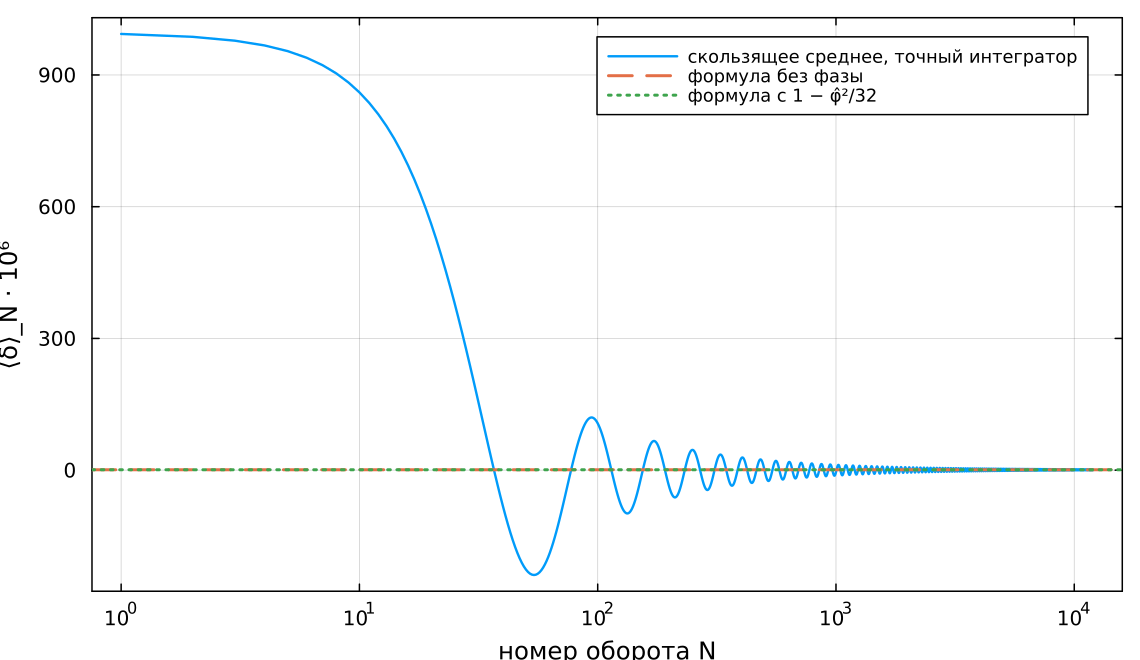
\includegraphics[width=0.92\textwidth]{figs/fig_03_phase.png}
\caption{Формула без фазы $\vMoneA$, с фазой $\vMonePhi$, сдвиг $\vPhaseShift$. Среднее интегратора к формуле с фазой: $\vDiffPhiMean$.}
\end{figure}

\textbf{Вывод.} Сдвиг уровня $\vPhaseShift$. На этих оборотах он сравни́м с остатком скользящего среднего, отдельной посадки на новую линию не видно.
